% !TEX TS-program = lualatex
% !TEX encoding = UTF-8

% This is a  template for creating an oversize initial in gregorio + latex.

\documentclass[12pt]{article} % use larger type; default would be 10pt
\usepackage{geometry} % See geometry.pdf to learn the layout options. There are lots.
\geometry{a4paper} % or letterpaper (US) or a5paper or....
\usepackage{gregoriotex} % for gregorio score inclusion
\usepackage{fullpage} % to reduce the margins
\usepackage[oldstyle]{libertine} % a font I like
\usepackage{lettrine} %for big initials in text outside of the chant scores
\usepackage{titlesec} %change the look of titles
\usepackage{graphicx}

% red colour
\definecolor{benred8}{HTML}{E82C00}

% FORMAT SUBSUBSECTIONS - use titlesec package
\titleformat{\subsubsection}{\centering\normalfont\color{benred8}}{}{1em}{}
\titlespacing{\subsubsection}{0 mm}{0 mm}{0 mm}

% SPACE BETWEEN Capitulum AND BIBLE VERSE
\def\capitulumSpace{\hspace{20 mm}}

% MAKES Ps : TEXT
\def\psalm{\textit{\textcolor{benred8}{Ps :}}}

% MAKES ALL \GreStars RED
\let\OldGreStar\GreStar
\renewcommand{\GreStar}{\textcolor{benred8}{\OldGreStar}}

% MAKES ALL \gredaggers RED
\let\OldGreDagger\GreDagger
\renewcommand{\GreDagger}{\textcolor{benred8}{\OldGreDagger}}

% MAKES ALL \Vbars RED
\let\oldVbar\Vbar
\def\VVbar{\textcolor{benred8}{\oldVbar\oldVbar .}}
\renewcommand{\Vbar}{\textcolor{benred8}{\oldVbar .}}

% MAKES ALL \Rbars RED
\let\oldRbar\Rbar
\renewcommand{\Rbar}{\textcolor{benred8}{\oldRbar .}}

% MAKES ALL \Abars RED
\let\oldAbar\Abar
\renewcommand{\Abar}{\textcolor{benred8}{\oldAbar .}}

% MAKES T.P. TEXT
\def\TemporePaschale{\textit{\textcolor{benred8}{T. P.}}}

% RESPONSE ENVIRONMENT
\newenvironment{response}{\leftskip 0in \setlength{\parindent}{0in}}{\vspace{2 mm}}

%%%%%%%%%%%%
% DOCUMENT %
%%%%%%%%%%%%

\begin{document}

\pagestyle{empty}

\begin{center}
	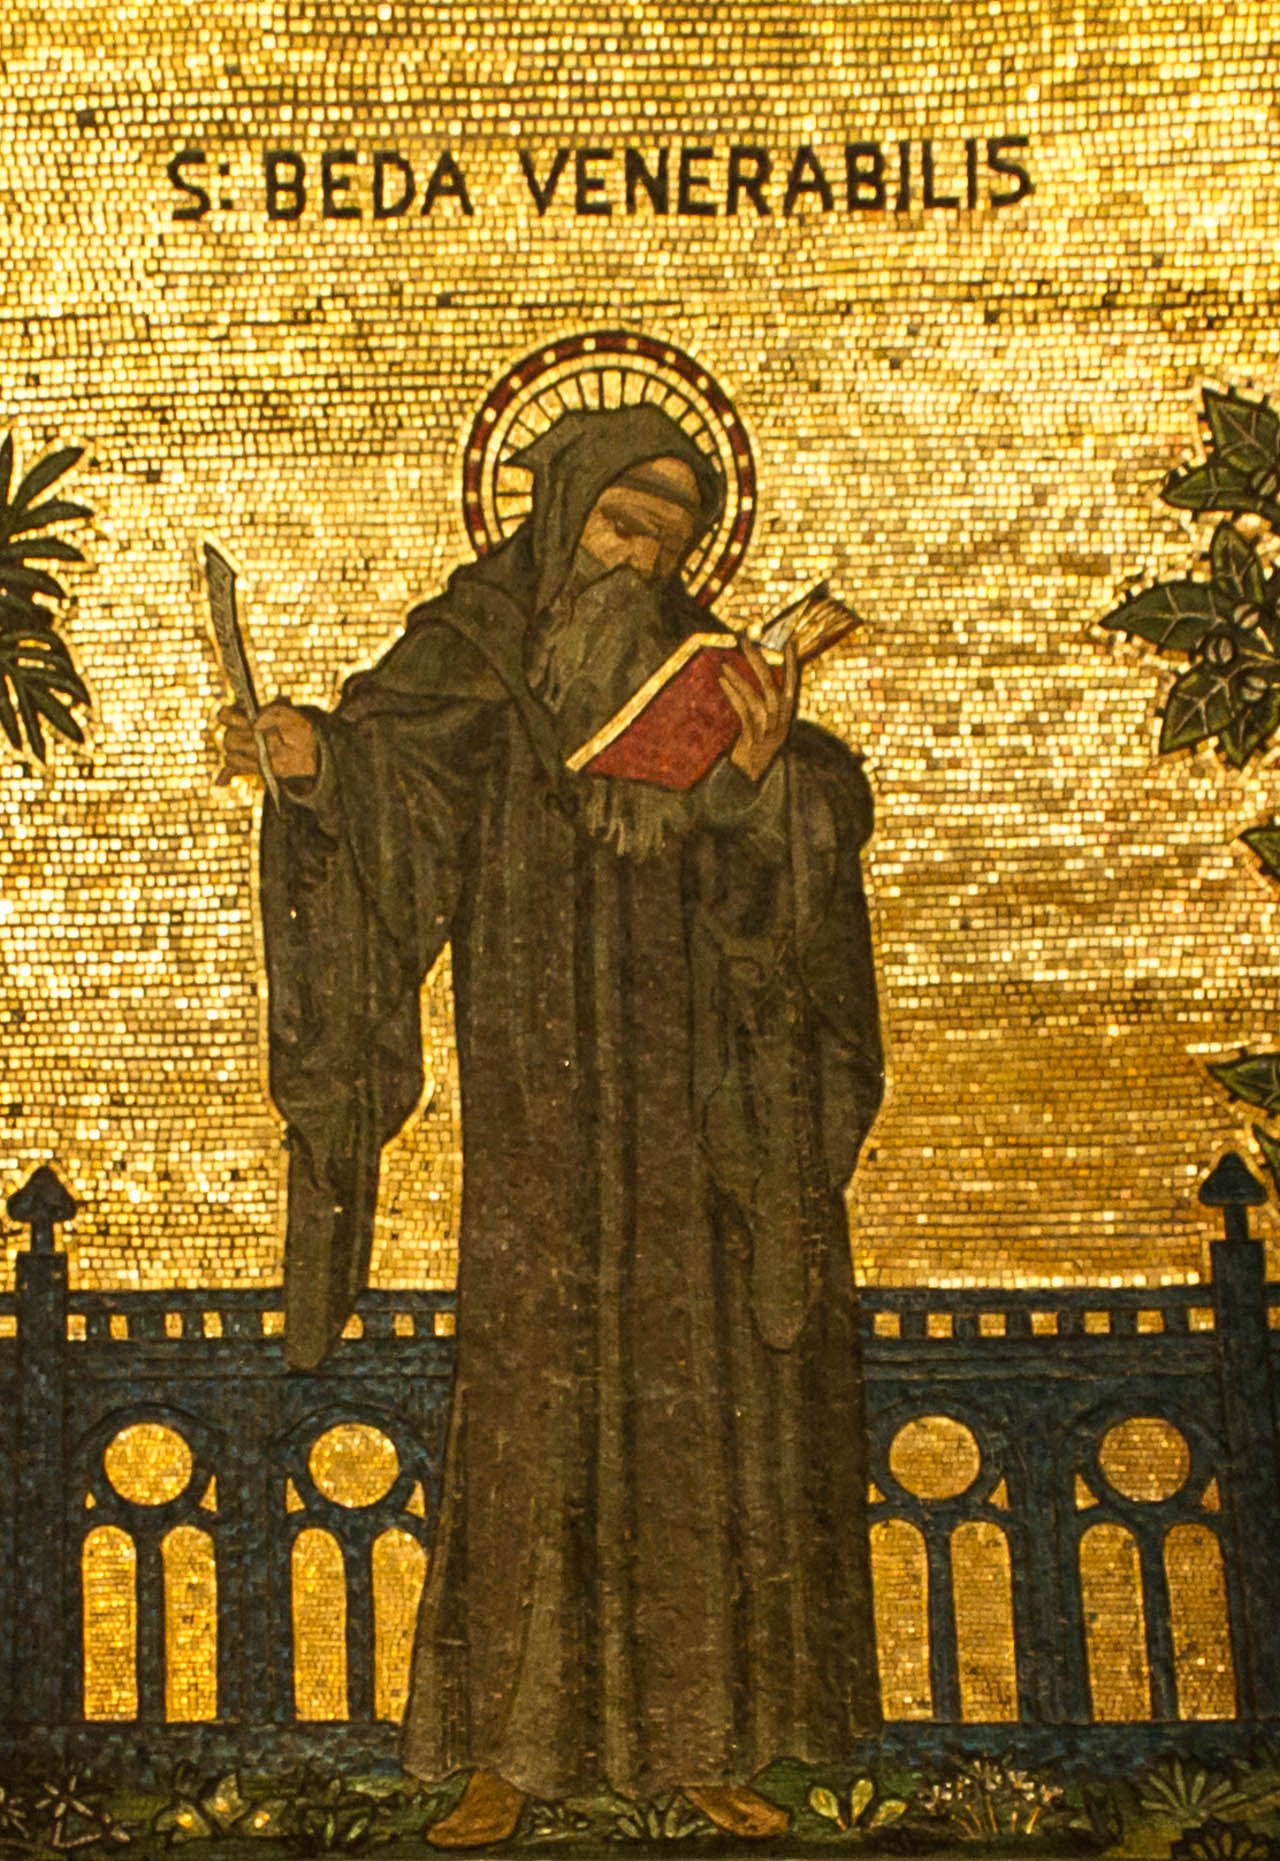
\includegraphics[width=8.5cm]{Saint-Bede-the-Venerable.jpg}

	\vspace{0.5cm}

	\begin{Large}\textsc{\textcolor{benred8}{Commemoratio de Sancto Beda.}}\end{Large}
\end{center}

\grechangestyle{annotation}{\color{benred8}}
\gregorioscore[a]{odoctoroptime_score.gtex} % a = compile gabc files if necessary

\begin{response}
	\Vbar\ Am\'{a}vit eum D\'{o}minus, et orn\'{a}vit eum.

	\Rbar\ Stolam gl\'{o}ri\ae\ \'{i}nduit eum.
\end{response}

\subsubsection*{\textcolor{black}{Or\'{e}mus.}\capitulumSpace \emph{Oratio.}}

\begin{response}
\lettrine{D}{e}us, qui Eccl\'{e}siam tuam be\'{a}ti Bed\ae\ Confess\'{o}ris tui atque Doct\'{o}ris eruditi\'{o}ne clar\'{i}ficas~:~\GreDagger\ conc\'{e}de prop\'{i}tius f\'{a}mulis tuis, \GreStar\ ejus semper illustr\'{a}ri sapi\'{e}ntia et m\'{e}ritis adjuv\'{a}ri. Per~D\'{o}minum nostrum Jesum Christum F\'{i}lium tuum : qui tecum vivit et regnat in unit\'{a}te Sp\'{i}ritus Sancti Deus, per \'{o}mnia s\'{\ae}cula s\ae cul\'{o}rum. \Rbar\ Amen.

\end{response}

\end{document}
